\section{Vulnerability: Oauth Redirect Attack}
\label{sec:background}
\textbf{Description:} The \verb|handleAuth| function in \verb|AuthController| is used to handle \textit{Oauth} redirects to another site. This means that any site is able to use
Wondough login page as a way for their customers to login to their website. Wondough however, has no checks on the redirect addresses that are allowed to use it. As such it is
possible for the user to be redirected back to a malicious site but with an access token intended for a legitmate site. Therefore it is possible to send key information an attacker
should not have access to, through the redirecting of urls. As such the attacker who set up the malicious website an access token to gain access to the user's account of a legitmate
website. Since this websie could be anything and as such potentially very important this is a very serious secuirty flaw.\\ \\
\textbf{Testing the Vulnerability:} In order to test this I checked to see if a redirect occurs for all sites and if a token is returned. I started with the dcs website by signing
into my Wondough account under the following url.
\begin{minted}{text}
http://localhost:39476/auth?app=1&target=http://warwick.ac.uk/fac/sci/dcs/
\end{minted}
As expected I was redirected with a token. This confirmed that this vulnerability could be exploited by an attacker through a malicious website and redirect attack. I retried this
but with other websites such as \verb|www.google.co.uk|, \verb|www.amazon.co.uk| and \verb|www.bbc.co.uk|. It worked with all of them. As such it was clear that no whitelist 
existed to allow Wondough to prevent malicious sites from using this feature. \\ \\
\textbf{Mitigation:} These attacks are prevented through the use of whitelists, whereby a site will submit an application to Wondough, requesting that it's site be able to use
Wondough's login page as a way for their users to sign in. As such Wondough would be able to assess the site ensure they were happy with its legitimacy and if so then add its url
to a whitelist. As such for the purposes of fixing Wonodugh I have created a whitelist, onto which I added the Wondough website and dcs:
\begin{minted}{java}
    private static String[] safeSites
        = {"http://localhost:1464/oauth",
        "https://warwick.ac.uk/fac/sci/dcs/"};
\end{minted}
Before this I had changed the port that the client side runs on to exclusively 1464 in order to whitelist it.\\ \\
\textbf{PLEASE NOTE:} if the \textit{sample-client} is not running on port 1464 the automated test won't pass and the website will not work either.\\ \\
I then edited the \verb|handleAuth| function to only reroute whitelisted ips. To do this I created a boolean function to return whether or not the parameter was a whitelisted url:
\begin{minted}{java}
    public static boolean trustedURL(String url){
        for (int i = 0; i < safeSites.length; i++) {
            if(url.equals(safeSites[i])) return true;
        }
        return false;
    }
\end{minted}
Then in the final part of \verb|handleAuth|, the site only redirects if \verb|trustedURl| returns true for the url. Otherwise the model has an error added to it informing that the
website isn't trusted so that the user can understand why the redirect didn't go through.
\begin{minted}{java}
    if(trustedURL(getQueryLoginRedirect(request))){
        response.redirect(
        getQueryLoginRedirect(request) + "?token=" +
        URLEncoder.encode(config.md5(app.getRequestToken()), "UTF-8")
        );
    }
    else{
        model.put("error", getQueryLoginRedirect(request)
        + " isn't a trusted website");
    }
\end{minted}
The choice to use and array and create the function \verb|trustedURl| was to ensure that it was inredibly easy for Wondough to add further urls withot having to change the code. All
that is needed is for another element to be added to \verb|safeSites[]|.\\
With this issue fixed it was then necessary to devise an automted test for it. This test would make use of HTTP status codes. If wondough directed you to an external site (not localhost:1464)
the code would be 302 (wihtout the fix). This means that the client has been told to look at (browse to) another URL. Whereas after the fix the code returned upon redirection would
be 200 (Standard response for successful HTTP requests)\cite{http}. Therefore the use of \verb|httpURLConnection| was used for the test to return the status codes of a whitelisted and
non whitelisted site and ensure they were appropriate. The first part of the test initialises the connection, sets it type to \verb|POST| (so that \verb|handleAuth| is called), and sets its \verb|doOutput| to true (allowing later the sending of a request body).
\begin{minted}{java}
    URL url = new URL("http://localhost:"+ Spark.port() + "/auth?");
    HttpURLConnection con = (HttpURLConnection)url.openConnection();
    con.setRequestMethod("POST");
    con.setDoOutput(true);
\end{minted}
From here a new \verb|DataOutputStream| is declared and the value is set to the output stream of the connection. The rest of the request is then added. This includes the username, password,
appname and. This is then written using \verb|writeBytes|. Finally the status of the request is gathered and compared to its expected value.
\begin{minted}{java}
    int status = con.getResponseCode();
    con.disconnect();
    if(status != 200) return "FAILED";
\end{minted}
This is repeated for both a url from the whitelist and one not from it. If both pass the test is considered successful. The test passes everytime after the fix having failed before, thus
the vulnerability can be considered eradicated.\\ \\
\textbf{PLEASE NOTE:} without the fix for this vulnerability the test will fail as expected but it will also throw an error. This can be ignored and the skeleton code will still
run as expected. The test still correctly failed:
\begin{figure}[h]
    \centering
    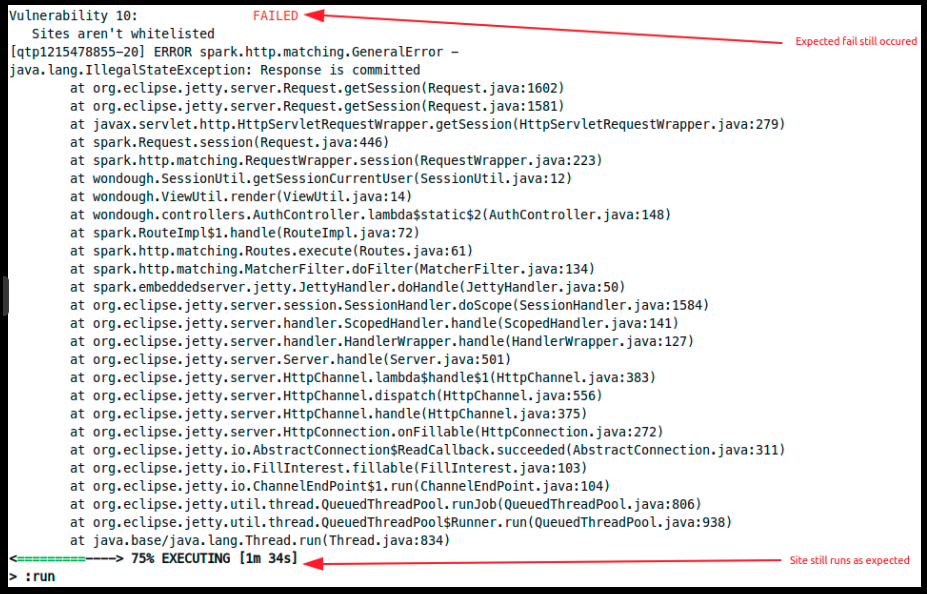
\includegraphics[width=1\textwidth]{figs/fail.png}
    \caption{The error thrown after the test fails on skeleton code}
    \label{10}
\end{figure}\\


